The purpose of limits is to find what a function approaches at a certain number that it is not defined for. 
For example, let's say we have the function $f(x) = \frac{x^2}{x}$ and $x = 0$ in this particular case. 
Since we are not allowed to divide by zero, this function is not defined there. 
However, the function may approach a certain number.

\begin{figure}[H]
\caption{Function approaching $1$ as $x$ goes to $0$}
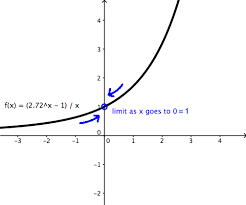
\includegraphics[scale=0.8]{../images.png}
\end{figure}

In the above graph, while the function is not defined at $0$, it approaches, or comes near to, $1$. 
There are several different "types" of limits and rules for calculating them. 

The first type of limit you could call an "easy" limit. 
All you have to do is plug in the number you are approaching for your variable, because the function doesn't violate any rules like we described above. 
So for example, if you have the limit

\begin{equation*}
    \lim\limits_{x\rightarrow 1} x
\end{equation*}

You would just get 1. 
The second type of limit could be called a "$\frac{0}{0}$" limit. 
It does violate the rules, and we have to do some algebraic manipulation to get it into a form we can work with. 
This might be done via factoring a polynomial, normalizing the denominator or numerator, or some such method.

A quick algebra side-note here on how to do these things. 
Factoring a polynomial mainly references factoring quadratics, or equations of the form $ax^2 + bx + c$ ($=0$). 
We factor the left side by using this general method: find the factors of $ac$ and see which add up to $b$. 
Note that you can change the signs of the factors, that is, if you have $ac = 10$ and the factors are $1, \, 2, \, 5, \, 10$, and $b = 3$, you can do $5-2 = 3$. 
After this, we then take those two numbers, $5$ and $-2$ and rewrite it as $ax^2 + 5x -2x + c$. 
We then put parentheses in: $(ax^2 + 5x) + (-2x + c)$. 
Finally, we factor out the biggest common number (or variable) out of each of the parentheses.

Let's do this with a real problem. 
\begin{equation*}
    x^2 - x - 12
\end{equation*}
For $ac$, we get $1\times -12$, or $-12$. 
For $b$, we get $-1$. 
The factors of $12$ are $1, \, 2, \, 3, \, 4, \, 6, \, 12$. $-4\times 3 = -12$ and $-4+3 = -1$. 
So now we write 
\begin{equation*}
    x^2 - 4x + 3x - 12
\end{equation*}
Now, we put in the parentheses and get
\begin{equation*}
    (x^2-4x)+(3x-12)
\end{equation*}
Now for the last step, factoring. 
For the first parenthesis, we can take out $x$, and in the second parenthesis, we can take out $3$, so we get
\begin{equation*}
    x(x-4)+3(x-4)
\end{equation*}
Note that if the two parenthesis' contents are not the same, then you have done something wrong. 
Now, we can rewrite this expression as 
\begin{equation*}
    (x+3)(x-4)
\end{equation*}
The equation is now factored.

The other thing of note here is rationalizing the denominator or numerator. 
Normally, we rationalize the denominator to get a radical out of the denominator, but we can also do this for the numerator. 
To do this, we multiply by expression on the numerator or the denominator over itself. 
Let's say we have the expression $\frac{\sqrt{x}}{1}$. 
Then we would multiply by $\frac{\sqrt{x}}{\sqrt{x}}$ and simplify. 
Note that if instead we had an expression like $\frac{\sqrt{x}+1}{1}$ we would multiply by $\frac{\sqrt{x}-1}{\sqrt{x}-1}$. 
We switched the sign on the $1$ from $+$ to $-$. This is called taking the "conjugate" of the expression.

With these tools in hand, we can now start solving the second type of limit. 
Let us take as an example 
\begin{equation*}
    \lim\limits_{x\rightarrow -3}\frac{x^2-x-12}{x+3}
\end{equation*}
We can clearly see that if we just plug it in, there will be a zero in the denominator. 
Instead, we can try employing an algebraic tool. 
You might recognize the quadratic on the top as the one we factored earlier. 
Let us then replace that expression with its factored form:
\begin{equation*}
    \lim\limits_{x\rightarrow -3}\frac{(x+3)(x-4)}{x+3}
\end{equation*}
Now, we can cancel the $x+3$ on the top and bottom of the fraction. 
This then leaves us with
\begin{equation*}
    \lim\limits_{x\rightarrow -3}x-4
\end{equation*}
The limit is now one of our "easy" limits, so we can simply plug in $-3$. The answer is $-7$.

Now we have our final type of limit, the "$\frac{\text{not zero}}{0}$" limit. 
This type of limit is a bit different from the other two types of limits. 
It requires a bit more intuition. As an example, let's say we are trying to solve the problem
\begin{equation*}
    \lim\limits_{x\rightarrow 0}\frac{1}{x}
\end{equation*}
To solve this, we must first solve
\begin{equation*}
    \lim\limits_{x\rightarrow 0^+}\frac{1}{x}
\end{equation*}
and
\begin{equation*}
    \lim\limits_{x\rightarrow 0^-}\frac{1}{x}
\end{equation*}
First, let's examine the second problem. 
The $+$ sign means it is a right limit - that is, we are approaching zero from the left. 
What does that mean? Well, let's say we have a number line like the one below.

\begin{figure}[H]
\caption{Approaching zero}
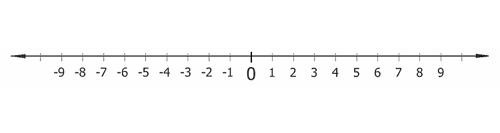
\includegraphics[scale=0.75]{../numberline.jpg}
\end{figure}

To approach from the right means that $x$ will be represented by tiny positive numbers, like $0.00001$ and $0.0000001$. 
They will get closer and closer to $0$. 
So, what does this mean? 
It means the answer to this particular limit will be whatever $\frac{1}{\text{really small positive number}}$ is. 
So let's take some examples. 
If we have $\frac{1}{0.00001}$ we get $100000$. 
If we have something closer to zero, like $\frac{1}{0.0000001}$ we get $10000000$. 
In other words, we are approaching infinity.
So the answer to this limit, approached from the right, is $+\infty$, or just $\infty$. 
Now, let's do the next one. 
This time, we are approaching zero from the left. Now we are dividing by small negative numbers. Try a few on a calculator and see what you get!

It turns out that this approaches $-\infty$. 
So the answer to the third limit in that list we started with is $-\infty$. 
Now, to solve the first limit. 
If we take the second two limits and their answer is the same, the first limit has a solution: the answer to the second two limits! 
However, the second two limits had different solutions. That means the answer to the first limit is undefined.
